\documentclass[12pt]{article}


\usepackage{charter}
\usepackage{fullpage}
\usepackage[colorlinks=false]{hyperref}
\usepackage{ifthen}
\usepackage{comment}
\usepackage[title,titletoc]{appendix}
\usepackage{pagecolor}
\usepackage{amsmath}
\usepackage{amsfonts}
%\usepackage[normalem]{ulem}
\usepackage{siunitx}
\usepackage{amsthm}
\sisetup{per=slash, load=abbr}

\usepackage{pgfplots}
\usetikzlibrary{positioning}
\usetikzlibrary{fit}
\usetikzlibrary{snakes}
\usetikzlibrary{shapes.geometric}
\usetikzlibrary{patterns}
\usetikzlibrary{shapes,arrows,chains}
\usepgfplotslibrary{patchplots,colormaps}
\usetikzlibrary{calc}
\usetikzlibrary{positioning, fit}
\usetikzlibrary{backgrounds}
\usetikzlibrary{intersections}

\newcommand{\whitepaper}[1]{\begin{center}\fbox{\parbox{0.75\textwidth}{{\small
#1}}}\end{center}}

\newcommand{\pcolor}{yellow!25}

\usepackage{setspace}
\usepackage{algorithm2e}
\bibliographystyle{ieeetr}

\usepackage{geometry}
\geometry{left=3cm,right=3cm,top=1.6cm,bottom=3cm,headheight=0pt,headsep=1.5em}
\usepackage{fancyhdr}
\pagestyle{fancy}
\chead{\includegraphics[scale=0.2]{../common/Nebulas.png}}  %在此处插入logo.pdf图片 图片靠左
\lhead{} % 页眉中间位置内容
\rhead{}
%\setlength{\topskip}{1em}

\usepackage{indentfirst}


\newcommand{\reffig}[1]{Fig.~\ref{#1}}
\newcommand{\refsec}[1]{~\S~\ref{#1}}


%\setlength{\parindent}{2.1em}
%\setlength{\parskip}{0.3\baselineskip}
\newcommand{\nrcore}{Core Nebulas Rank}
\newcommand{\nrext}{Extended Nebulas Ranks}
\newcommand{\nr}{Nebulas Rank}
\newcommand{\dom}{{\; \texttt{dom}\;}}

\onehalfspacing

\newtheorem{property}{Property}
%\addbibresource{reference.bib}

\begin{document}
\pagestyle{empty}
%\renewcommand{\nomname}{术语表(按首字母排序)}
%\renewcommand{\baselinestretch}{1.5}

\pagecolor{\pcolor}

\begin{titlepage}
  \begin{center}
    \vspace*{5.5cm}
    \includegraphics[scale=0.5]{../common/Nebulas.png}
    \vspace{0.5cm}


    \textbf{\huge{Yellow Paper: Nebulas Rank}}

    \vspace{0.5cm}
    Nebulas Research
    \vfill
    June 2018\\
    Version:1.0.1
    \textbf{}
  \end{center}

\end{titlepage}
\setcounter{page}{0}
%\thispagestyle{empty}
\tableofcontents
\newpage
\setcounter{page}{1}
\pagestyle{fancy}
\vspace*{0.01cm}
\section{概要}

一般而言,在传统的软件开发行业,开发者在某开发平台
(如Windows\footnote{\url{https://www.microsoft.com/en-us/windows}},Linux\footnote{\url{https://en.wikipedia.org/wiki/Linux}},
macOS\footnote{\url{https://en.wikipedia.org/wiki/MacOS}},
iOS\footnote{\url{https://en.wikipedia.org/wiki/IOS}},
Android\footnote{\url{https://en.wikipedia.org/wiki/Android}}等)上开发相应的应用,并由此获利。
开发者的获利方式主要包括,薪资、售卖自己主导或参与开发的软件以及在免费分发的软件中插入广告流量。

然而,应用平台方在软件的使用中所获得的利益并没有被公平的分配给相应的开发者。例如,某用户需要使用Sketch而不得不购买搭载macOS的Mac设备\footnote{\url{https://www.sketchapp.com/support/requirements/other-platforms/}},
并由此付出费用,尽管Sketch的开发者可以向用户收取使用费用,
但是通过售卖Mac设备而获利的Apple公司\footnote{\url{https://en.wikipedia.org/wiki/Apple_Inc.}}并不会因此额外向Sketch的开发者分享利益;类似的,某用户需要使用AutoCAD\footnote{\url{https://en.wikipedia.org/wiki/AutoCAD}}软件时,只能选择搭载macOS或Windows的设备,
由此需要支付给Apple或Microsoft\footnote{\url{https://en.wikipedia.org/wiki/Microsoft}}及相关企业
的费用亦并未向AutoCAD的开发者分享。
诚然, 用户选择一个平台的原因多种多样,其中一个关键性的影响因素是需要的应用所支持的平台,换句话说,一个应用平台的发展,离不开其上的优秀应用。
因此,应用平台方无视开发者利益的做法,一定程度上侵害了开发者的利益。

在区块链中,去中心化应用(Decentralized Application, DApp)开发者的利益同样被漠视。
2014年,以太坊提出在区块链上运行图灵完备的智能合约(Smart Contract),使得区块链从单纯的数字货币支付网络升级为了去中心化应用平台。
然而,DApp开发者的获利方式与传统的软件开发行业相比,并无明显区别,即,开发者并不能从去中心应用平台或区块链系统的发展中获利。

可以抽象的认为,区块链中出块奖励代表了区块链系统发展中新增的价值,而出块奖励的分发决定了去中心化系统的激励方向。我们认为,区块链系统增加的价值本质上来源于新增的用户数据所蕴含的价值,这些新增的价值
应该公平的分发给为系统的新增价值做出贡献的各方,其中,就包括DApp开发者。然而,在以比特币为代表的区块链系统中,出块奖励被发放给了矿工节点;在诸多的基于PoS(Proof of Stake)的区块链系统中,
出块奖励被发放给了系统代币的持有者;同样的,在诸多的区块链系统中,DApp开发者的利益一定程度上都被漠视或侵害了。

一般而言,一个去中心化应用可以理解为为了实现特定功能的一系列智能合约的集合。
智能合约是一种旨在以信息化方式传播、验证或执行合同的计算机协议。智能合约允许在没有第三方的情况下进行可信交易\footnote{\url{https://en.wikipedia.org/wiki/Smart\_contract}}。
从技术架构来看,大部分DApp通常以智能合约作为后端,同时采用了常见的前端技术与之交互,因此DApp形态既可以是传统个人电脑客户端,也可以是移动应用或者网页应用。

我们认为,去中心化应用平台、DApp开发者及DApp用户,这三者是互相促进的。
首先,去中心化应用平台的出现,扩大了区块链开发者这一群体,越来越多的开发者尝试开发满足不同需求的DApp,并从DApp的开发中获益;
其次,DApp开发者提供了丰富多样的DApp,扩大了区块链的应用场景,为区块链带来了更多的用户;
最后,DApp用户驱动着去中心化应用平台的不断的优化、升级,增加去中心化应用平台之上代币的流通性,是的整个区块链系统得以发展。
因此,更进一步的,我们认为,DApp开发者的利益应该得到公平的分配,并给予保证,这是区块链做为去中心化应用平台维持可持续发展的关键所在。

需要注意,本文所述的开发者仅指去中心化应用平台之上的DApp开发者,不特指星云链上的DApp开发者,亦不包括区块链系统本身的开发者,因此,如无歧义,下文所述的开发者皆指DApp开发者。
特别的,DApp开发者在身份上可能同时持有一定数量的代币,而DApp开发者因为持币而带来的任何收益都不能等同的认为享受到了区块链系统发展带来的增值,
其做为DApp开发者的利益依然可能是被漠视甚至侵害的。


让应用开发者在平台的发展中公平获益,在技术上并不容易实现。一方面,在传统的软件开发行业中,平台的发展及获利状况及由中心化的组织掌握,平台之上的应用开发者无从知晓或参与相应的利益分配;
另一方面,应用开发者为平台发展所做出的贡献难以量化,利益分配难以做到公平公正。
而在区块链为基础的去中心化应用平台上,这一状况有望得到改善。区块链的价值来源于代币的流通性,DApp的使用情况被公开的记录在区块链上,得益于此,\textbf{基于DApp的使用情况,
量化DApp的使用对一个区块链系统的发展所做出的贡献,并进一步给予开发者公平的激励},是必要且可行的。

理想情况下,对于DApp开发者的激励需要满足如下基本性质:
\begin{itemize}
\item 公平性:对于DApp开发者的激励,需要保证相对客观,即每个DApp需要被公平的对待,其使用情况需要被真实的衡量,并摒弃可能存在的操纵行为。
\item 有效性:对于DApp开发者的激励,需要真实反映用户的偏好,即获得激励高的DApp是活跃用户所喜欢且经常使用的,而获得激励低的DApp是鲜有用户问津的。
\begin{comment}
	\item 公开性:链上的DApp激励协议与传统的评奖方式最大的不同在于,所有评分的机制必须是完全公开的,
	且其中任何统计、计算、评选的过程都是全程可见的。
	这样就杜绝了传统中心化评奖暗箱操作的可能。同时也不会出现票数统计出错等情况。
	最后,根据评选结果分配奖励的过程也会保证被执行,奖励分配正如链上交易一样可被追溯。
	\item 有效性:这也是任何评选机制所要满足的基本性质。我们期望DApp评分能够真实反映用户的评价,
	即排名高的DApp是活跃用户所喜欢的且经常被调用的,而评分低的DApp是用户鲜有问津的。
	\item 抗作弊:对于任何排名算法,都需要解决各类作弊问题。对于DIP而言,主要存在两类作弊问题。
	\begin{enumerate}
		\item 女巫攻击:区块链技术的一个重大特点就是一个用户建立新的节点地址代价是很小的。所以一个用户有可能建立多个由他控制的地址,并将他们伪装成多个正常用户来参与评选。
		一个好的激励协议应当保证每个用户无法通过女巫攻击带来巨大额外收益。
		\item 收买:由于我们衡量DApp好坏的主要指标是活跃用户调用的次数,一个DApp开发者有可能收买大量用户让他们调用自己的DApp以提高自己的排名从而获得更多奖励。
		这种作弊方式原则上无法杜绝,但我们期望激励协议能够让此类收买需要付出的代价变得很高以减少其出现的概率。
	\end{enumerate}
\end{comment}
\end{itemize}


本文提出DApp开发者激励协议(Developer Incentive Protocol,DIP),试图给予开发者激励,让DApp开发者能够公平的在去中心化应用平台的发展中获益。
我们深知,用户对于DApp的真实评价是主观且多维的,一个理想的DApp开发者激励协议可能是不存在的,因此,本文给出的DApp开发者激励协议依然存在各种不足,
其中仍然包含了我们对于DApp开发者的偏好。然而,在抵抗操纵及保证开发者利益之间,本文所做出的权衡依旧是创新性的,即,在保证DApp开发者利益的前提下,在抵抗操作方面,做出了最大限度的努力。

本文提出的开发者激励协议基于已有的星云指数(Nebulas Rank)~\cite{Nabulasyellowpaper},由于星云指数的相关性质,开发者激励协议能够在一定程度上很好的保证上述性质。
直观的来说,开发者激励协议将用户对DApp的使用情况简化为用户根据自己的喜好对DApp进行投票的问题,用户的投票总数为该用户的星云指数,而对DApp的使用则为对DApp的投票,
最终根据投票结果,对开发者给予相应比例的激励。

本紫皮书在给出开发者激励协议的理论模型之外,还对其抵抗操纵的性质进行了分析,并对系统中如何实现开发者激励协议给出了必要的说明,例如,如何对开发者激励协议进行必要的调整及更新,
从而对开发者激励协议的实际落地给出了具体的工作方向。

\whitepaper{
特殊提示:
本开发者激励协议紫皮皮书作为专项讨论开发者激励协议的紫皮书,对星云技术白皮书(2018年4月发布的1.02版本)~\cite{Nabulas}中开发者激励协议相关章节进行了大幅度的升级和拓展。
相对于一年前的概念论证,经过一年的深入思考与实际验证,我们有信心和能力设计出更为严谨的算法,并对星云指数的更多实际细节问题提供明确的解决方案或方向。
为了方便阅读,我们将使用实线框高亮解释技术白皮书提及过、并且在本紫皮书中有升级的相关技术点。
}

\section{Antecedentes}
\label{sec:antecedentes}
\noindent
El protocolo tratado en este libro púrpura se basa en un gran número de trabajos relacionados, y además completa o actualiza la información previamente disponible. En esta sección trataremos esas obras relacionadas, que jugaron un rol significativo como referencia y guía para la confección de este libro púrpura.

\subsection{Incentivos para el desarrollo de aplicaciones descentralizadas}
\noindent
Por lo que sabemos, en la actualidad ninguna plataforma descentralizada basada en blockchains ofrece
mecanismos de incentivos a largo plazo para desarrolladores de {\dapp}s. En su papel de representantes de la blockchain 2.0, Ethereum supuso un gran avance al implementar contratos inteligentes Turing-completos: en su red aparecieron distintas aplicaciones,
incluyendo juegos, apuestas, sistemas de \textit{crowd sourcing}, préstamos, créditos, entre otros. En particular, el juego de \textit{tokens} coleccionables CryptoKitties —a fines de 2017— y Fomo3D —en 2018— atrajeron la mayor atención.

En la actualidad, y tal como sucede con los ejemplos descriptos en el párrafo anterior, la mayoría de los desarrolladores de {\dapp}s obtuvieron sus utilidades únicamente a través del cobro de comisiones a sus usuarios, sin que les resultara posible beneficiarse del incremento del valor de Ethereum o de las recompensas por nuevos bloques.

Con esta falta de incentivos para los desarrolladores, el escenario de las aplicaciones descentralizadas también se vio afectado. Por ejemplo, implícitamente, puede existir una carencia total de DApps gratuitas debido a la dificultad de obtener ingresos por medio de ellas. Como resultado de esto, la cantidad, la calidad y la diversidad de {\dapp}s se ve afectada. En contraste, la implementación de un mecanismo efectivo para incentivar a los desarrolladores logra el propósito de atraerlos al ecosistema del desarrollo de {\dapp}s, lo que promueve la prosperidad y el desarrollo del ecosistema blockchain.

Hasta cierto punto, muchos sistemas blockchain emergentes comprenden la necesidad de implantar mecanismos de incentivos para construir sus ecosistemas. Por ejemplo, en el programa \textit{Nebulas Incentive}, se desarrollaron más de 6781 DApps, y también se logró que un gran número de equipos de desarrollo puedan obtener beneficios de esas DApps de forma directa.

En paralelo, otros blockchains públicos lanzaron también programas de incentivos a corto plazo basados en una administración centralizada. Tales programas apuntan principalmente a publicitarse entre la comunidad, aunque con evaluaciones oficiales tomando un rol central, sin sustentabilidad a largo plazo.


\subsection{Nebulas Rank}
\noindent
Nebulas Rank (NR)\cite{Nebulasyellowpaper} cuantifica la contribución de cada cuenta al rendimiento económico total, y provee características para impedir la manipulación en las mediciones. En particular, Nebulas Rank introduce la \textbf{función Wilbur}, que tiene las siguientes propiedades:

\begin{property}
	\label{prop:one}
	Para dos variables positivas dadas $x_1$,$x_2$, la suma de sus funciones es menor que la función de su suma.
	%对于任意输入$x$,将其拆分后的计算函数之和小于原计算函数。
\end{property}
\begin{align}
	f(x_1+x_2)>f(x_1)+f(x_2) \quad x_1>0,x_2>0
\end{align}
\begin{property}
	\label{prop:two}
	Para dos variables positivas dadas $x_1$,$x_2$, cuando estas tienden a infinito, la suma de sus funciones tiende a la función de su suma.
\end{property}

\begin{align}
	\lim\limits_{x_1 \to \infty, x_2\to \infty} f(x_1+x_2) = f(x_1) + f(x_2)\quad x_1>0, x_2>0
\end{align}
\noindent Como base de NR, estas dos propiedades ofrecen también resistencia contra la manipulación.

\subsection{Mecanismos de voto}
\noindent
Como se mencionó antes, el proceso por el cual los usuarios eligen y utilizan las {\dapp}s disponibles se puede ver como una forma de votar por ellas en el protocolo DIP. El mecanismo de los incentivos es similar al algoritmo de valuación (\textit{ranking}). Con respecto a estos dos últimos, existen numerosos trabajos relacionados en distintos campos; a continuación brindaremos una muestra de ellos.

Uno de los estudios más famosos es el teorema de Arrow, que sostiene que, cuando los votantes tienen tres o más alternativas, no es posible crear un sistema de votación que refleje las preferencias de los votantes en una \textit{preferencia global} mientras se satisfacen tres condiciones: independencia de alternativas irrelevantes (que la valuación relativa de dos candidatos no se vea afectada por la de un tercer candidato), ausencia de \textit{dictadores} (que ningún candidato o individuo tenga el poder de cambiar las preferencias del grupo), y eficiencia de Pareto\footnote{Dada una asignación inicial de bienes en un grupo de individuos, una redistribución de esos bienes que mejora la situación de un individuo, sin hacer que empeore la situación de los demás, se denomina eficiencia de Pareto} (el resultado de la valuación satisface los intereses de la mayoría). El estudio implica que ningún algoritmo de valuación puede cubrir todas las posibilidades. Así, el Protocolo de Incentivos para Desarrolladores que se discute en este libro púrpura se enfocará en los atributos más importantes y conocidos.

En la vida real existe un sinnúmero de escenarios que requieren algoritmos de valuación. Un ejemplo claro para esta afirmación es la reputación dada por los compradores a los vendedores de Amazon, Taobao y otros sitios similares. Los vendedores con mayor reputación obtendrán mejor exposición en la plataforma, y gracias a ello obtendrán más visibilidad y mayor tasa CTR\footnote{\textit{Click Through Rates}, o tasa de clics.}. En
particular, existen problemas similares en estas plataformas de comercio electrónico, como el ataque Sybil\footnote{Ataque que consiste en crear transacciones falsas para obtener revisiones de cinco estrellas.}.

Por el momento, esas plataformas centralizadas dependen mayormente de la capacidad de aprendizaje de sus sistemas para distinguir entre transacciones normales y falsas\cite{mukherjee2013spotting,jindal2008opinion,yoo2009comparison}.
De todas maneras, la práctica demostró que tales métodos no son los ideales.
\cite{ott2011finding} señala que incluso la identificación mediante inteligencia artificial no puede distinguir entre ambas cuentas con efectividad. \cite{cai2016mechanism} expone un algoritmo que elimina el incentivo para tales manipulaciones basadas en el diseño del mecanismo. Aun cuando ese modelo difiere del nuestro, es posible utilizarlo como una referencia significativa.

\cite{salihefendic2010hacker} introduce un algoritmo de valuación para publicaciones en redes sociales que combina los votos de los usuarios y la declinación del tiempo.

\cite{salihefendic2010reddit} introduce un algoritmo de valuación para publicaciones en la red social Reddit, que implica una situación en la que los usuarios pueden emitir votos negativos.

\cite{miller2009how} introduce el algoritmo de valuación de comentarios de la red social Reddit, que toma en cuenta el intervalo de confianza.

IMDB~\cite{IMDB} presenta la idea de un Promedio Bayesiano de Modelos (BMA en inglés) para su sistema de valuación de filmes, que puede reducir la brecha entre las diferentes películas debido al número de votantes.

Gracias a las propiedades anti-manipulativas de NR, el Protocolo de Incentivos para Desarrolladores propuesto en este libro púrpura puede distinguir entre usuarios normales y usuarios falsos de una forma más clara. Así, el énfasis de este documento está en transferir el valor NR de los usuarios a los puntos de valuación de las {\dapp}s a través de comportamientos interactivos.
\input{economic.tex}
\section{DApp评分}
\begin{frame}
\frametitle{DApp评分}
“调用即投票”:
\begin{itemize}
	\item 用户调用行为在链上公开可见,无法篡改;
	\item 调用行为更能反映用户的真实使用情况。
\end{itemize}
\[
\Gamma_{ij} = \frac{e_{ij}}{e_{i0}+\sum_{j=1}^n {e_{ij}}} \Gamma_i
\]
\end{frame}

\begin{frame}
\frametitle{DApp评分}
开方排名分:
\begin{itemize}
	\item 用户调用越多的DApp其产生的投票效用越高,鼓励用户接触更多DApp;
	\item 有效防止开发者收买用户。
\end{itemize}
\[
S_j = g(\Gamma_{1j},\Gamma_{2j},...,\Gamma_{mj}) = \sum_{i=1}^m \sqrt{\Gamma_{ij}}
\]
\end{frame}

\input{core-anti.tex}
\input{core-impl.tex}
\section{未来工作}
\subsection{多维投票行为}
在~\ref{subsection:voting}小节中,我们采用了用户调用行为作为DApp排名参考依据,我们同时也给出了不采用调用过程中涉及的资金交互作为参考依据的原因。在未来工作中,在能够解析智能合约调用的情况下,我们可以更细粒度的区分调用过程中的资金转移原因,则可以尝试引入资金交互这一特性作为DApp排名参考依据。

\subsection{DApp之间的调用}
DApp的排名目前主要来自于用户的投票效用(即用户星云指数),这种传递过程来自用户调用合约行为。而更复杂的调用行为,例如智能合约直接的内部调用,也可能进一步传递用户投票效用。因此在接下来的工作中,我们可以给定所有DApp排名分初始值,随后根据DApp间调用关系图运行Page Rank算法~\cite{page1999pagerank}求得最终排名分。

%所有DApp的排名分定位page rank初始值,随后根据DApp间调用图运行page rank算法作为最终排名分。
\input{future.tex}
\newpage
\bibliography{reference}

\newpage
\begin{appendices}
\section{Pruebas}
\subsection{Prueba de propiedad \ref{p1}}
\label{subsection:proof1}
\begin{proof}
	Sin pérdida de la generalidad, podemos asumir que las \textit{ponderaciones} con los que el votante $a_i$
	valúa todas las {\dapp}s son $b_{i1}, b_{i2}, \ldots, b_{in}$ respectivamente, y que son valores fijos. Asumimos que los valores de contribución del votante $a_i$ a todas las {\dapp}s son
	$\nr_{i1},\ldots,\nr_{in}$ respectivamente, y que son ajustables por el votante $a_i$.

	El objetivo de la optimización del votante $i$ es la suma ponderada de los puntajes de las valuaciones que ofrece, definida por:
	$$w_i = \sum_{j=1}^n b_{ij}\sqrt{\nr_{ij}}$$
	De acuerdo a la inecualidad de Cauchy, se desprende que:
	$$w_i = \sum_{j=1}^n b_{ij}\sqrt{\nr_{ij}} \leq (\sum_{j=1}^n b_{ij}^2)(\sum_{j=1}^n \nr_{ij}) \leq (\sum_{j=1}^n b_{ij}^2)\nr_i$$
	El último término del segundo miembro en la ecuación de arriba es un valor fijo. La igualdad se mantiene sí y sólo sí:
	$$\frac{b_{i1}^2}{\nr_{i1}}=\frac{b_{i2}^2}{\nr_{i2}}=\cdots=\frac{b_{in}^2}{\nr_{in}}$$
	Así, la propiedad queda demostrada.
\end{proof}

\subsection{Prueba de propiedad \ref{p2}}
\label{subsection:proof2}
\begin{proof}
	Sin pérdida de la generalidad, se asume que el desarrollador de la dapp $d_1$ la divide en dos {\dapp}s. Para todo votante normal que pertenece al segundo caso descripto en la sección \ref{subsec:5.2} asumiendo que las \textit{ponderaciones} asignados a valuar las
	{\dapp}s antes de su división son $b_{i1},b_{i2},\ldots,b_{in}$ y las ponderaciones con los que valúa las dos {\dapp}s divididas son $b'_{i1},b'_{i2}$, se sostiene que $b_{i1} \geq b'_{i1}+b'_{i2}$ de acuerdo a nuestra presunción.

	Luego, computamos los valores de contribución del votante $a_i$ antes de ocurrir la división. Se define $H_i = \sum_{j=2}^n b_{ij}^2$, de acuerdo a la conclusión en la propiedad \ref{p1} y de acuerdo al Teorema de Particiones tenemos:
		 $$\frac{\nr_{i1}}{b_{i1}^2} = \frac{\sum_{j=1}^n \nr_{ij}}{\sum_{j=1}^n b_{ij}^2} = \frac{\nr_i}{b_{i1}^2+H_i}$$
  Similarmente, el valor de contribuciones del votante $a_i$ a la $t$-a división de la \dapp (denotada por $\nr'_{it},t=1,2$) es:
  	 $$\nr'_{it} =  \frac{b_{it}^{'2}\nr_i}{b_{i1}^{'2}+b_{i2}^{'2}+H_i}$$
  	 Nótese que $b_{i1}^2 \geq (b‘_{i1}+b’_{i2})^2 >b_{i1}^{'2}+b_{i2}^{'2}$, tenemos
  	 $$\nr_{i1} > \nr'_{i1}+\nr'_{i2}$$
  	 Así, introducimos la restricción de los valores de contribución para un votante lo suficientemente racional. Generalmente, la mayoría de los votantes pertenece al primer caso descripto en la sección \ref{subsec:5.2}, esto es, sencillamente distribuyen los valores de contribución que se suponen para $d_1$ para las {\dapp}s divididad. En cualquier caso, tenemos:
  	 	 	$$\nr_{i1} \geq \nr'_{i1}+\nr'_{i2}$$
  	 Defínase $S'_1,S'_2$ como los dos puntajes de valuación de las {\dapp}s, respectivamente. Por definición:
  	 	 $$S'_1 =  \sum_{i=1}^m \sqrt{\nr'_{i1}},~~~S'_2 =  \sum_{i=1}^m \sqrt{\nr'_{i2}},~~~S_1 = \sum_{i=1}^m \sqrt{\nr_{i1}}$$
  	Defínase $U'_1$ como el incentivo final del desarrollador de la \dapp $d_1$ luego de la división. Por definición:
  		 $$U'_1=\frac{S_1^{'2}+S_2^{'2}}{S_1^{'2}+S_2^{'2}+\sum_{j=2}^n S_j^2} \lambda M,~~~U_1=\frac{S^2_1}{S_1^2+\sum_{j=2}^n S_j^2} \lambda M$$
  	Nótese que dados $S_2,\ldots,S_n$,
  		 $$ U_1 \geq U'_1 \Leftrightarrow S_1^2 \geq S_1^{'2}+S_2^{'2}$$
   Para mostrar si la división aumenta la utilidad, sólo es necesario comparar los siguientes dos términos:
   	 $$S_1^2 = (\sum_{i=1}^m \sqrt{\nr_{i1}})^2,~~~S_1^{'2}+S_2^{'2}=  (\sum_{i=1}^m \sqrt{\nr'_{i1}})^2+(\sum_{i=1}^m \sqrt{\nr'_{i2}})^2$$
   	En realidad, $S_1^2 \geq S_1^{'2}+S_2^{'2}$ pueden ser demostrados de acuerdo al teorema de la distancia más corta.
   		 \begin{figure}
   		 	\centering
   		 	%\includegraphics[width = 0.6\textwidth]{../common/m1.png}
   		 	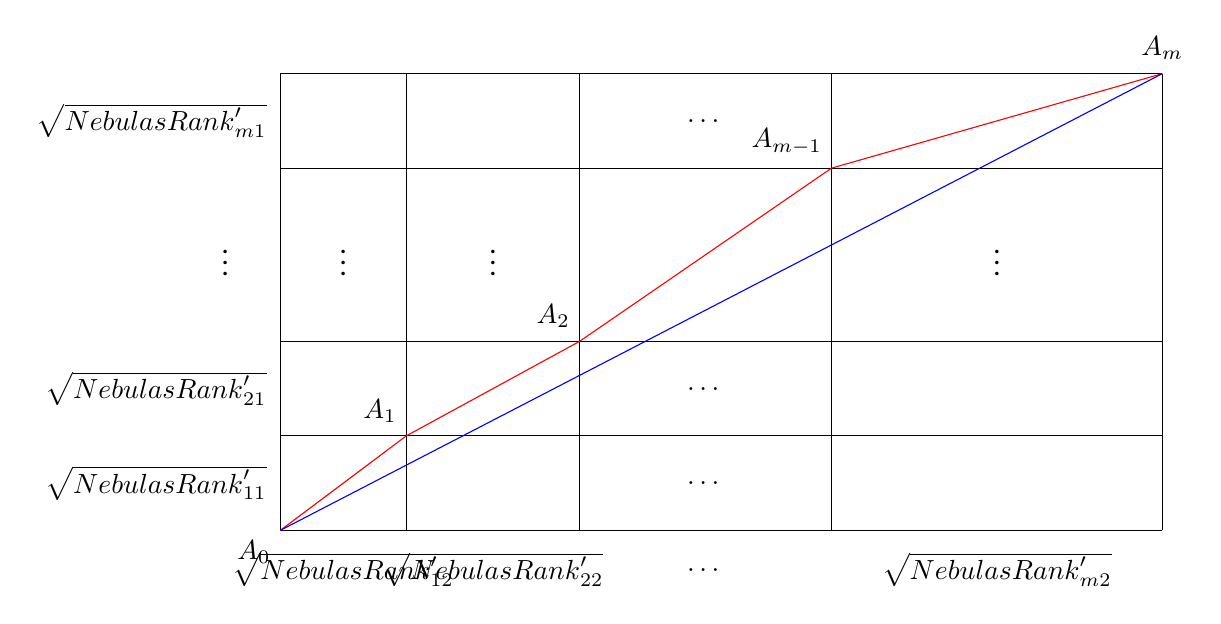
\begin{tikzpicture}
\pgfmathsetmacro{\HEIGHT}{1.2}
\pgfmathsetmacro{\HDOT}{2.2}
\pgfmathsetmacro{\WDOT}{3.2}
\pgfmathsetmacro{\WOne}{1.6}
\pgfmathsetmacro{\WTwo}{2.2}
\pgfmathsetmacro{\WN}{4.2}

\pgfmathsetmacro{\LEN}{\WOne + \WTwo + \WN + \WDOT}
\pgfmathsetmacro{\TH}{3*\HEIGHT+ \HDOT}

\tikzset{
  t/.style={draw, on grid, align=center, minimum height=1ex},
  coord/.style={coordinate, on grid, node distance=6mm and 25mm},
  between/.style args={#1 and #2}{
         at = ($(#1)!0.5!(#2)$)
    }
}

\draw [name path=h1] (0, 0) -- (\LEN, 0);
\draw [name path=h2] (0, \HEIGHT) -- (\LEN, \HEIGHT);
\draw [name path=h3] (0, 2*\HEIGHT) -- (\LEN, 2*\HEIGHT);
\draw [name path=h4] (0, 2*\HEIGHT + \HDOT) -- (\LEN, 2*\HEIGHT + \HDOT);
\draw [name path=h5] (0, 3*\HEIGHT + \HDOT) -- (\LEN, 3*\HEIGHT + \HDOT);

\draw[name path=v1] (0, 0) -- (0, \TH);
\draw[name path=v2] (\WOne, 0) -- (\WOne, \TH);
\draw[name path=v3] (\WOne + \WTwo, 0) -- (\WOne + \WTwo, \TH);
\draw[name path=v4] (\WOne + \WTwo + \WDOT, 0) -- (\WOne + \WTwo + \WDOT, \TH);
\draw[name path=v5] (\WOne + \WTwo + \WDOT + \WN, 0) -- (\WOne + \WTwo + \WDOT + \WN, \TH);

\path [name intersections={of=h1 and v1,by=A0}];
\path [name intersections={of=h2 and v2,by=A1}];
\path [name intersections={of=h3 and v3,by=A2}];
\path [name intersections={of=h4 and v4,by=Am1}];
\path [name intersections={of=h5 and v5,by=Am}];

\draw [red] (A0) -- (A1) -- (A2) -- (Am1) -- (Am);
\draw [blue] (A0) -- (Am);

\node [below=0.01 of A0, anchor=north east] {$A_0$};
\node [above=0.05 of A1, anchor=south east]{$A_1$};
\node [above=0.05 of A2, anchor=south east] {$A_2$};
\node [above=0.05 of Am1, anchor=south east] {$A_{m-1}$};
\node [above=0.05 of Am, anchor=south]{$A_m$};


\path [name intersections={of=h1 and v1,by=t00}];
\path [name intersections={of=h2 and v1,by=t01}];
\path [name intersections={of=h3 and v1,by=t02}];
\path [name intersections={of=h4 and v1,by=t03}];
\path [name intersections={of=h5 and v1,by=t04}];
\node [coord, between=t00 and t01] (x1){};
\node [coord, between=t01 and t02] (x2){};
\node [coord, between=t02 and t03] (x3){};
\node [coord, between=t03 and t04] (x4){};

\node [left=0.05 of x1.west] {$\sqrt{{\nr}'_{11}}$};
\node [left=0.05 of x2.west] {$\sqrt{{\nr}'_{21}}$};
\node [left=0.7 of x3.west, anchor=center] {$\vdots$};
\node [left=0.05 of x4.west] {$\sqrt{{\nr}'_{m1}}$};

\path [name intersections={of=h1 and v1,by=s00}];
\path [name intersections={of=h1 and v2,by=s01}];
\path [name intersections={of=h1 and v3,by=s02}];
\path [name intersections={of=h1 and v4,by=s03}];
\path [name intersections={of=h1 and v5,by=s04}];
\node [coord, between=s00 and s01] (y1){};
\node [coord, between=s01 and s02] (y2){};
\node [coord, between=s02 and s03] (y3){};
\node [coord, between=s03 and s04] (y4){};

\node [below=0.5 of y1.south, anchor=center] {$\sqrt{{\nr}'_{12}}$};
\node [below=0.5 of y2.south, anchor=center] {$\sqrt{{\nr}'_{22}}$};
\node [below=0.5 of y3.south, anchor=center] {$\dots$};
\node [below=0.5 of y4.south, anchor=center] {$\sqrt{{\nr}'_{m2}}$};

\node at (x1.east -| y3.north) {$\dots$};
\node at (x2.east -| y3.north) {$\dots$};
\node at (x4.east -| y3.north) {$\dots$};

\node at (y1.north |- x3.east) {$\vdots$};
\node at (y2.north |- x3.east) {$\vdots$};
\node at (y4.north |- x3.east) {$\vdots$};

\end{tikzpicture}

   		 	\caption{Prueba de la distancia más corta\label{fig:path}}
   		 \end{figure}
   Como se muestra en la figura \ref{fig:path}, construimos una grilla cuyos largo y ancho están divididos en $m$ segmentos, cuyo $i$-ésimo segmento tiene una longitud de $\sqrt{\nr'_{i1}}$ y $\sqrt{\nr'_{i2}}$ respectivamente.

   	Entonces, $S_1^{'2}+S_2^{'2}=A_0A_m^2$, esto es, es igual al cuadrado de la longitud del segmento azul. Entretanto,
   	 $$S_1^2 = (\sum_{i=1}^m \sqrt{\nr_{i1}})^2 > (\sum_{i=1}^m \sqrt{\nr'_{i1}+\nr'_{i2}})^2 = (\sum_{i=1}^m A_{i-1}A_i)^2$$,
   	 que es igual a la suma de los cuadrados de todos los segmentos rojos. Como la distancia más corta entre dos puntos es un segmento lineal, se mantiene que $S_1^2 >S_1^{'2}+S_2^{'2}$.

   	 Para los casos en los que las {\dapp}s $k>2$ están divididas, podemos considerarlo como divisiones sucesivas y usar iterativamente el resultado en $k=2$.

   	 Así, la propiedad queda probada.

\end{proof}

\subsection{Prueba de corolario \ref{c1}}
\label{subsection:proof3}
\begin{proof}
	Para todo votante comprado por el desarrollador de una \dapp $d_1$, antes de su división, podemos considerar al votante como un votante normal que valúa todas las {\dapp}s con un vector de ponderación $(1,0,0,\ldots,0)$, ya que otorga toda su capacidad de voto a $d_1$.
	Suponemos ahora que $d_1$ se divide en $k$ {\dapp}s y que los valores de contribución de los votantes comprados a las {\dapp}s $k$ son $\nr_{t1},\ldots,\nr_{tk}$, cuya suma es fija. De acuerdo a la condición de que la igualdad se mantenga para la inecualidad de Cauchy en la Prueba de Propiedad \ref{p1}, el votante puede ser considerado como un votante normal que valúa todas las {\dapp}s con un vector de ponderación
	$(\sqrt{\nr_{t1}}/C,\sqrt{\nr_{t2}}/C,\ldots, \sqrt{\nr_{tk}}/C,0,0,\ldots,0)$, donde $C=\sum_{j=1}^k \sqrt{\nr_{tj}}$. Esto es, el votante valúa las {\dapp}s divididas con ponderaciones de acuerdo a proporción, y valúa todas las otras {\dapp}s con ponderaciones 0.\footnote{Nótese que al escalar todas las ponderaciones mediante una constante no se afectan los resultados, ya que el valor de contribución total del votante sólo depende de las proporciones de las ponderaciones con respecto a las ponderaciones totales}. Como
		$$\sum_{j=1}^k \sqrt{\nr_{tj}}/C =1$$
	por lo que el caso de este corolario puede reducirse al caso de los votantes normales. (Propiedad\ref{p2}). Así, el corolario queda probado.
\end{proof}

\subsection{Prueba de propiedad \ref{p3}}
\begin{proof}
	Consideramos en primer lugar el caso de un votante que divide su cuenta en dos sub-cuentas. Consideramos $c$ como la cuenta original y $a,b$ como las sub-cuentas, $S,S'$ son las puntuaciones de valoración de la \dapp que el votante planea votar antes y después de la división respectivamente, $U,U'$ son los incentivos finales para el desarrollador de la \dapp que el votante planea votar, antes y después de la división respectivamente. Por definición, tenemos
	$$S= \sqrt{\nr_c}+O,\quad S'=\sqrt{\nr_a}+\sqrt{\nr_b}+O$$,
	donde $O$ es la suma de los valores de contribución de otros votantes, que es un valor fijo.

	Mediante ~\ref{eq:sqrt_nr} se sostiene que $S < S'$. Esto es, la valuación de la \dapp no se incrementa.

	Entretanto, por definición,
	$$U = \frac{S}{S+P}\lambda M,\quad U' = \frac{S'}{S'+P} \lambda M$$,
	donde $P$ es la suma de los cuadrados de los puntajes de la valuación de las otras \dapp, cuyo valor es fijo.

	Como $S < S'$ se sostiene que $U \leq U'$. Esto es, el incentivo final que recibe el desarrollador no se incrementa.

	Para los casos en los que $k>2$ cuentas están divididas, podemos considerarlo como divisiones sucesivas y usar iterativamente el resultado en $k=2$.

\end{proof}
\section{Change log}
\subsection{2019.4.8 change log}
\begin{itemize}
	\item Replace the function from NR to capacities (\ref{eq:capacity}) by  $f(\mathcal{C}(a_i))=\mathcal{C}(a_i)$
	\item Replace the calculation of the participation factor $\lambda$ (\ref{eq:participation}) by $\min\{\frac{0.008}{1-r},1\}$, where $r=\frac{\nr_p}{\nr_s}$
	\item Fix typos.
\end{itemize}
\subsection{2019.5.27 change log}
Fix several typos.
\end{appendices}

\end{document}
